%%%
\documentclass[xcolor=dvipsnames, aspectratio=169]{beamer}
%\usepackage{beamerthemesplit, listings, verbatim}

%\usepackage[absolute,overlay,showboxes]{textpos}
\usepackage[absolute,overlay]{textpos}

\usepackage{fontspec}

\usepackage{graphicx,wrapfig}
\usepackage{amsfonts,amsmath, amssymb, latexsym, amsthm}
\usepackage{epsfig}
\usepackage{float,enumerate}
\usepackage{listings}
\usepackage{mathtools}
\usepackage{multicol}
\usepackage{pifont}
\usepackage{tikz}
\usepackage{tikz-3dplot}
\usetikzlibrary{arrows}
\usepackage{ulem}
\usepackage{xcolor}


\definecolor{Blueprint}{RGB}{0,61,162}
\definecolor{DarkBlue}{rgb}{0.15,0.0,0.9}
\definecolor{Red}{rgb}{0.9,0.0,0.1}
\definecolor{Red2}{rgb}{0.49,0.0,0.02}
\definecolor{Colortest}{rgb}{0.1,0.55,0.1}
\definecolor{Orange}{rgb}{0.75,0.3,0.3}
\definecolor{JBlue}{HTML}{08399F}
\definecolor{Purple}{HTML}{8243DB}
\definecolor{aocbg}{HTML}{0F1022}
\definecolor{aocfg0}{HTML}{1FCA23}
\definecolor{aocfg1}{HTML}{106319}

\setbeamertemplate{navigation symbols}{} % turns nav syms off
\setbeamercolor{background canvas}{bg=Red2}


%\title[Daily Notes]{A Beamer Template for notes}
%\subtitle[]{}
\author[JLP]{Jesse L. Patsolic}


\def\Title#1{\noindent{\large\textcolor{gray!50}{\sf{#1}}}}
\def\MTitle#1{\noindent{\large\textcolor{gray!50}{\tt{#1}}}}

\newcommand\Mygrid{%
\tikz[
  remember picture,
  overlay,
  color=white,
  yscale=-1,
  xstep=\TPHorizModule,ystep=\TPVertModule,
  yshift=\TPVertModule,xshift=0pt]
  \draw (current page.north west) grid (current page.south east);}

\begin{document}

%% Example of a full page figure.
\begin{frame}[plain]
%	\Mygrid
%\begin{textblock}{11}(0,0)
%    \Title{Jesse Leigh Patsolic, B.S., M.A.}
%\end{textblock}
%\makebox[\linewidth]{\includegraphics[height=0.95\paperheight]{logoBig.png}}

%%% Middle Explainer Box
%\begin{textblock}{5}(5,4)
%	\MTitle{%
%	Consider the case where $\{A, A_1\}$ are synonyms and $\{A,B\}$ are a pair of keywords.
%	}
%\end{textblock}

\begin{textblock}{3}(1,1)
    \MTitle{
	\begin{tabular}{l} 
	\href{https://oeis.org/A250001}{A250001:}  Number of
	    arrangements of n circles in the affine plane.\\ 
	    Kissing not allowed.\\
	    \begin{tabular}{ l | l | l | l | l | l | l}
		n & 0 & 1 & 2 & 3 & 4 & 5\\
		\hline
             a(n) & 1 & 1 & 3 & 14 & 173 & 16951
	    \end{tabular}
	\end{tabular}
}%
\end{textblock}

\begin{textblock}{5}(1,5)
	
\begin{tikzpicture}[scale=0.5, color = gray!50, line width=1]
		\draw (-2.25,0) circle (1cm);
		\draw (0,0) circle (1cm);
		\draw (2.25,0) circle (1cm);
	\end{tikzpicture}
\end{textblock}

\begin{textblock}{5}(5,5)
	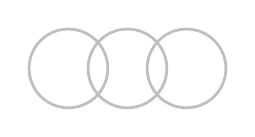
\begin{tikzpicture}[scale=0.5, color = gray!50, line width=1]
		\draw (-1.5,0) circle (1cm);
		\draw (0,0) circle (1cm);
		\draw (1.5,0) circle (1cm);
	\end{tikzpicture}
\end{textblock}


\begin{textblock}{5}(8,5)
	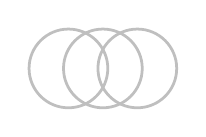
\begin{tikzpicture}[scale=0.5, color = gray!50, line width=1]
		\draw (-0.875,0) circle (1cm);
		\draw (0,0) circle (1cm);
		\draw (0.875,0) circle (1cm);
	\end{tikzpicture}
\end{textblock}

\begin{textblock}{5}(11,5)
	
\begin{tikzpicture}[scale=0.5, color = gray!50, line width=1]
	        \draw (-0.5,0) circle (1cm);
		\draw (0,0) circle (7mm);
		\draw (0.5,0) circle (1cm);
	\end{tikzpicture}
\end{textblock}


\begin{textblock}{5}(8,8)
	
\begin{tikzpicture}[scale=0.5, color = gray!50, line width=1]
		\draw (0,0) circle (1cm);
		\draw (0,0) circle (4mm);
		\draw (2.1,0) circle (1cm);
	\end{tikzpicture}
\end{textblock}


\begin{textblock}{5}(11.5,8)
	
\begin{tikzpicture}[scale=0.5, color = gray!50, line width=1]
		\draw (0,0) circle (1cm);
		\draw (-0.25,0) circle (4mm);
		\draw (0.25,0) circle (4mm);
	\end{tikzpicture}
\end{textblock}


\begin{textblock}{5}(13,8)
	
\begin{tikzpicture}[scale=0.5, color = gray!50, line width=1]
		\draw (0,0) circle (1cm);
		\draw (-0.375,0) circle (3mm);
		\draw (0.375,0) circle (3mm);
	\end{tikzpicture}
\end{textblock}


\begin{textblock}{5}(1,8)
	
\begin{tikzpicture}[scale=0.5, color = gray!50, line width=1]
		\draw (0,0) circle (1cm);
		\draw (-0.5,0) circle (3mm);
		\draw (1,0) circle (1cm);
	\end{tikzpicture}
\end{textblock}


\begin{textblock}{5}(3,8)
	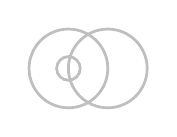
\begin{tikzpicture}[scale=0.5, color = gray!50, line width=1]
		\draw (0,0) circle (1cm);
		\draw (0,0) circle (3mm);
		\draw (1,0) circle (1cm);
	\end{tikzpicture}
\end{textblock}

\begin{textblock}{5}(5.5,8)
	
\begin{tikzpicture}[scale=0.5, color = gray!50, line width=1]
		\draw (-0.5,0) circle (1cm);
		\draw (0,0) circle (3mm);
		\draw (0.5,0) circle (1cm);
	\end{tikzpicture}
\end{textblock}



\begin{textblock}{5}(12,11)
	
\begin{tikzpicture}[scale=0.5, color = gray!50, line width=1]
		\draw (0,0) circle (1cm);
		\draw (0,0) circle (6.5mm);
		\draw (0,0) circle (3mm);
	\end{tikzpicture}
\end{textblock}

\begin{textblock}{5}(1,11)
	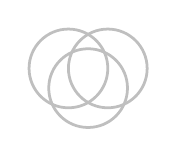
\begin{tikzpicture}[scale=0.5, color = gray!50, line width=1]
		\draw (-0.5,0.5) circle (1cm);
		\draw (0.5,0.5) circle (1cm);
		\draw (0,0) circle (1cm);
	\end{tikzpicture}
\end{textblock}


\begin{textblock}{5}(5,11)
	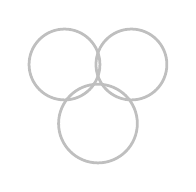
\begin{tikzpicture}[scale=0.5, color = gray!50, line width=1]
		\draw (-0.85,1.5) circle (9mm);
		\draw (0.85,1.5) circle (9mm);
		\draw (0,0) circle (1cm);
	\end{tikzpicture}
\end{textblock}


\begin{textblock}{5}(8,11)
	
\begin{tikzpicture}[scale=0.5, color = gray!50, line width=1]
		\draw (-2.25,0) circle (1cm);
		\draw (0,0) circle (1cm);
		\draw (1.5,0) circle (1cm);
	\end{tikzpicture}
\end{textblock}



\end{frame}


\end{document}
%%%
%%% TIME: 
%%% WORKING STATUS:
%%% COMMENTS:
